\documentclass{article}
\usepackage{full page, listings, graphicx, cprotect, csquotes, hanging, hyperref, cleveref, mathtools}
\usepackage[labelfont=bf]{caption}
\lstset{
numbers=left, 
numberstyle=\small, 
numbersep=8pt, 
frame = single, 
language=Java, 
framexleftmargin=15pt}
\newenvironment{nscenter}
 {\margin=0.5pt\parskip=0pt\par\nopagebreak\centering}
 {\par\noindent\ignorespacesafterend}
% set the document title, author, and date here.
%  once set, the \maketitle command (within the document)
%  will display them nicely
\title{Mazewrold}
\author{Mauricio Esquivel Rogel}

\begin{document}
\maketitle

\section{Introduction}
This particular solution of Mazeworld provides full functionality for two situations of a single-robot maze: 
\begin{enumerate}
  \item A non-blind robot
  \item A blind robot
\end{enumerate}
This includes mazes of all sizes as long as their width  \verb`mazeWidth` and height  \verb`mazeHeight` are both more than or equal to 4 for the reasons covered in \cref{sec:model}. However, the model does provide the instance variables and functions necessary to implement multiple robots and PAC-MAN physics, all that's missing is time. The extension that took most of my time was implementing the most efficient way to do an \verb`A* search` with a Fibonacci Heap, so I had to neglect some other extensions of the project. I also focused on creating a graphical representation of the maze that's more aesthetically pleasing than simple ASCII code (see \autoref{fig:unsolved} for an example of a 20x20 maze without solutions).  Furthermore, this solution provides flexibility with selecting initial positions and goals, as illustrated in \cref{sec:model} as well.

\begin{figure}[!htb]
\label{fig:unsolved}
\centering
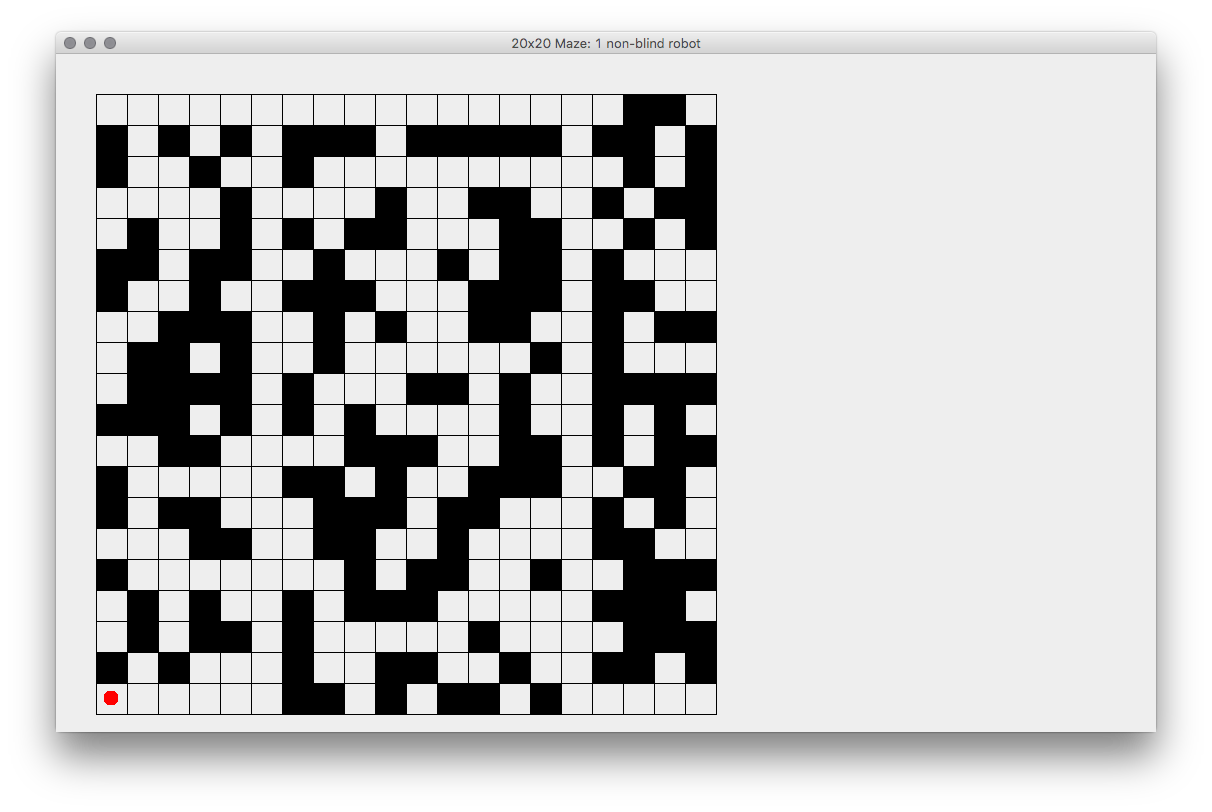
\includegraphics[width=1\linewidth]{./figures/maze20x20.png}
\cprotect\caption{An example of an unsolved 20x20 maze with one robot at $(0, 0)$. The black squares represent obstacles and white squares represent available paths.}
\end{figure}

This program implements \verb`Breadth-First` and \verb`A*` search algorithms and finds optimal solutions, even with blind robots. In this solution, the only difference between a blind robot scenario vs a non-blind robot scenario is that in the former, the robot does not know its initial position. In this case, states actually become belief states, and a belief state  $b_i$ takes the form $b_1 = [s_1, s_2, ..., s_i]$ where $i$ represents the number of states it contains and $s_k$ a particular physical state of the robot agent. Since these mazes are two-dimensional, a physical state $s_r$ is defined to be $s_r = (x, y, d, r)$  where $x$ and $y$ are the coordinates of $s_r$ in the maze's Cartesian plane, $d$ is $s_r$'s depth from the initial position, and $r$ is the \verb`id` of the robot. This solution doesn't use robot \verb`id`s because it can only handle one robot at a time, but it's there for further development. When the robot is not blind, belief states become a single physical state of the same form.

An upper bound $B_u$ for the total number of physical states for a maze with a single non-blind robot would be 
\[
  B_n = \verb`mazeWidth` * \verb`mazeHeight`,
\]
disregarding the legality of states, where $n$ stands for non-blind. Therefore, by the space complexity analysis of belief states given in page of {\it Artificial Intelligence: A Modern Approach}, an upper bound $B_b$ for the total number of physical states for a maze with a single non-blind robot would be 
\[
  B_b = 2^{B_n},
\]
disregarding the legality of states, where $b$ stands for blind this time.

\section{Running the program}
\label{sec:driver}
The driver \verb`MazeworldDriver.java` can run tests and then proceed with the finding the solution, or simply skips the first step. This is determined by the \verb`TESTING` constant on top of the file:
\begin{lstlisting}
  // TESTING TOGGLE 
  public static final boolean TESTING = true;   // ACTIVATE
//  public static final boolean TESTING = false;  // DEACTIVATE
\end{lstlisting}
Clearly, this configuration tells the driver to run all tests as specified in \cref{sec:testing}. Then the driver generates a random 50x50 maze with a non-blind robot and solves it first with \verb`Breadth-First Search`and then with \verb`A* Search`. Once it has concluded, it goes on to create another random 50x50 maze this time with a blind robot and solves it with \verb`A* Search`. This is the default set-up, but it is in no way unique. I have tested the maze with values up to \verb`mazeWidth = mazeHeight = 400` with successful results, but there's nothing to suggest that 400 is the actual upper bound. These are the console results from that run:\\
\begin{lstlisting}
Breadth-First Search
Path length:  1198 [(0,0), (1,0), (2,0), (3,0), (4,0), ... ]
Nodes explored during last search:  2141069
Maximum memory usage during last search 2144737
Running time: 29.776s
--------
A* Search
Path length:  1198 [(0,0), (1,0), (2,0), (3,0), (4,0), ...]
Nodes explored during last search:  629391
Maximum memory usage during last search 633669
Running time: 13.807s
--------
\end{lstlisting}
To be safe, choose widths and heights according to these bounds:
 \[
   3 < \verb`mazeWidth` , \text{ and }
 \] 
 \[
   3 < \verb`mazeHeight`,
 \]
\cref{sec:model} explains where these bounds come from. Also, you have to fix $y$ and $gy$ to $0$ and select values for $x$ and $gx$ according to these bounds to ensure an optimal solution:
  \[
   0 \leq \verb`x` < \lfloor \verb`mazeWidth` / 4 \rfloor , \text{ and }
 \]
 \[
    3 * \lfloor \verb`mazeWidth` / 4 \rfloor \leq  \verb`gx` < \verb`mazeWidth`,
\]
 also covered in \cref{sec:model}.
 
\section{Testing}
\label{sec:testing}
The \verb`MazeworldTest.java` creates various instances of verb`PriorityFibonacciHeap`and checks the output to make sure that it works. These are the tests:

\begin{lstlisting}
private boolean IntegerTest1() {  
    PriorityFibonacciHeap<IntegerKey> fibHeap = 
        new PriorityFibonacciHeap<IntegerKey>(new IntegersComparator());
    for (int i = 0; i < 50; i++) {
      fibHeap.insert(new 
          FibonacciHeapNode<IntegerKey>(new IntegerKey(49 - i)));
    }
    
    for (int i = 0; i < 50; i++) {
      if (fibHeap.poll().getValue().intValue() != i) {
        failedTests++;
        return false; 
      }
    }
    
    if (!fibHeap.isEmpty()) { 
      failedTests++;
      return false; 
    }
    
    return true;
  }
  
  private boolean IntegerTest2() {
    PriorityFibonacciHeap<IntegerKey> fibHeap = 
        new PriorityFibonacciHeap<IntegerKey>(new IntegersComparator());
    int expectedInt = 0;
    
    for (int i = 0; i < 50; i++) {
      fibHeap.insert(new 
          FibonacciHeapNode<IntegerKey>(new IntegerKey(i)));
      
      if (i % 5 == 0) {
        if (fibHeap.poll().getValue().intValue() != expectedInt) {
          failedTests++; 
          return false; 
        }
        
        expectedInt++;
      }
    }
    
    while (!fibHeap.isEmpty()) { 
      if (fibHeap.poll().getValue().intValue() != expectedInt) {
        failedTests++; 
        return false; 
      }
      
      expectedInt++;
    }
    
    return true;
  }
\end{lstlisting}

This is the sample output of all tests passing:

\begin{lstlisting}
Test 1: Check if after inserting integers 0 to 49
in reverse order to the heap, all of them can be extracted
until the heap is empty
PASSED

Test 2: Check if after inserting integers 0 to 49
in order to the heap, all of them can be extracted
at different times until the heap is empty
PASSED

ALL TESTS PASSED
\end{lstlisting}

\section{Implementation of the model}\label{sec:model}
The model is implemented in  \verb`MazeworldProblem.java`. All problems have the same constructor:\\
\begin{lstlisting}
public MazeworldProblem(int nrobots, int w, int h, int gx,   
      int gy, boolean b, boolean pP) {
    totalRobots = nrobots;
    mazeWidth = w;
    mazeHeight = h;
    goalx = gx;
    goaly = gy;
    blindRobots = b;
    pacmanPhysics = pP;
    robots = new RobotNode[totalRobots];
    startNode = new ArrayList<UUSearchNode>();
    
    if (this.blindRobots)
      beliefStates = new ArrayList<ArrayList<UUSearchNode>>();
    
    mazeWalls = loadMaze();
    mazePanel = new JPanel();
    
    if (mazeFrame == null) {
      mazeFrame = new JFrame();
      mazeFrame.setBackground(Color.WHITE);
    }
    
    if (mazePanel == null) {
      mazePanel = new JPanel();
      mazePanel.setBackground(Color.WHITE);
    }
    
    mazeFrame.setTitle(w + "x" + h + (this.pacmanPhysics ? 
        " Pacman-Physics" : "") + " Maze: " + nrobots + " " +
        (this.blindRobots ? "blind" : "non-blind") + " robot" +
            (nrobots == 1 ? "" : "s"));
    
    for (int i = 0; i < totalRobots; i++) {
      this.robots[i] = new RobotNode(0, i, 0, i);
      
      if (blindRobots) { beliefStates.add(predict(INIT_MOVE, i)); }
      
      this.startNode.add(this.robots[i]);
    } 
    
    startMaze();
  }
\end{lstlisting}

\verb`blindRobots` specifies whether the only robot is blind and \verb`pacmanPhysics` would be the variable responsible of implementing the PAC-MAN world. Given any problem, the first function that gets called is \verb`loadMaze`:\\

\begin{lstlisting}
private int[][] loadMaze() {
    int[][] maze = new int[this.mazeWidth][this.mazeHeight];
    Random random = new Random();
    
    int midpointWidth = Math.floorDiv(this.mazeWidth, 2);
    int lowerQuartileWidth = Math.floorDiv(midpointWidth, 2);
    int upperQuartileWidth = midpointWidth + lowerQuartileWidth;
    
    for (int h = 0; h < this.mazeHeight; h++) {
      for (int w = 0; w < this.mazeWidth; w++) {
        if (h == 0) {
          if (w <= lowerQuartileWidth || w >= upperQuartileWidth)
            maze[w][h] = 1;
        } else if (h < this.mazeHeight - 1) {
          if (w == lowerQuartileWidth || w == upperQuartileWidth)
            maze[w][h] = 1;
        } else {
          if (w <= upperQuartileWidth)
            maze[w][h] = 1;
        }
      }
    }
    
    for (int w = 0; w < this.mazeWidth; w++) {
      for (int h = 0; h < this.mazeHeight; h++) {
        if (maze[w][h] != 1) {
          maze[w][h] = (random.nextBoolean()) ? 1 : -1;
        }
      }
    }
    
    return maze;
  }
\end{lstlisting}
This function randomly creates a maze with only one constraint: create an open path (a solution) from $(0,0)$ to  $(\lfloor \verb`mazeWidth` / 4 \rfloor , 0)$ to $(\lfloor \verb`mazeWidth` / 4 \rfloor , \verb`mazeHeight`)$ to to $(3 * (\lfloor \verb`mazeWidth` / 4 \rfloor) , \verb`mazeHeight` - 1)$ to $(3 * (\lfloor \verb`mazeWidth` / 4 \rfloor) , 0)$ and finally to $(\verb`mazeWidth` - 1 , 0)$. This ensures that the bounds mentioned in \cref{sec:driver} guarantee a solution.

\section{Priority Fibonacci Heap}
Given this \verb`minHeap` version's impressive running time, I decided it would be best to implement \verb`A* Search` with it. According to Professor Cormen's {\it Algorithms} book, three of the operations that concern \verb`A* Search` (creation, \verb`insert()`, and \verb`decreaseKey()`) run in constant time, and only \verb`poll()` runs in logarithmic time. Priority Fibonacci Heap implements directly the pseudocode in Professor Cormen's {\it Algorithms} book for Fibonacci Heap. This is the code for the public methods in \verb`PriorityFibonacciHeap.java`,\\
\begin{lstlisting}
//-------------------------------- insert() ----------------------------//
  /*
   * Adds a new node to the heap.
   * @param newNode - node to be added 
   */
  public void insert(FibonacciHeapNode<E> newNode) {
    // if heap is empty, make this new node be the only element in a new
    // root list
    if (this.min == null) { this.min = newNode; }
    
    // otherwise, splice it into the root list and update min if necessary 
    else {
      this.min.spliceRight(newNode);
      
      if (this.comparator.compare(newNode.getValue(),
          this.min.getValue()) == -1) {
                this.min = newNode;
            }
    }
    
    this.numberOfNodes++; 
  }

//---------------------------------- peek() ----------------------------//
  /*
   * Returns the min element without removing it from the heap.
   * @return min element 
   */
  public FibonacciHeapNode<E> peek() {
    return this.min;
  }
//---------------------------------- poll() ----------------------------//  
  /*
   * Returns and removes the heap's min element while "consolidating" the heap
   * i.e. rearranging the heap to satisfy the constraint. 
   * @return min element
   */
  public FibonacciHeapNode<E> poll() {
    FibonacciHeapNode<E> min = this.min, child = null, temp = null;
    
    // if the heap is not empty, extract the min element from the heap,
    // add any of its children to the root list, and consolidate if
    // necessary
    if (min != null) {
      child = min.childrenList;
      
      // splice min element's children into the root list
      while (min.degree > 0) {
        temp = child.right;
        
        child.spliceOut();
        this.min.spliceRight(child);
        
        child.parent = null;
        
        min.decreaseDegree();
        child = temp;
      }
      
      // extract min element
      min.spliceOut();
      
      // if min element was the only element, then there is no new min
      if (min == min.right) { this.min = null; }
      
      // otherwise consolidate heap starting with the element to the right
      // of the min element as the new min element
      else {
        this.min = min.right;
        consolidate();
      }
      
      this.numberOfNodes--;
    }
    
    return min;
  }

//------------------------------ decreaseKey() -----------------------------//
  /*
   * Returns and removes the heap's min element while "consolidating" the heap
   * i.e. rearranging the heap to satisfy the constraint. 
   * @param currNode - node already in heap whose key will be decreased
   * @param newKey - currNode's new key
   */
  public void decreaseKey(FibonacciHeapNode<E> currNode, double newKey) {
    FibonacciHeapNode<E> y = null;
    
    // if the newKey is bigger than the old one, so decreasing is
    // impossible
    if (newKey > currNode.getKey()) { return; }
    
    // update old key to new key
    currNode.setKey(newKey);
    
    // get the node's parent and check if there are changes to be made
    y = currNode.parent;
    
    // if changes are in order, rearrange the heap back into structure
      if (y != null &&
          this.comparator.compare(currNode.getValue(),
              y.getValue()) == -1) {
        cut(currNode, y);
          cascadingCut(y);
      }
  
      // update min if necessary
      if (this.comparator.compare(currNode.getValue(), 
          this.min.getValue()) == -1) {
        this.min = currNode;
      }
  }
  
//-------------------------------- delete() ----------------------------//
  /*
   * Forces an element to be polled out of the heap. 
   * @param node - node to be deleted
   */
  public void delete(FibonacciHeapNode<E> node) {
    // make node new min and extract it as usual
        decreaseKey(node, Double.NEGATIVE_INFINITY);
        poll();
    }

//-------------------------------- size() ------------------------------//
  public int size() {
    return this.numberOfNodes;
  }

//-------------------------------- isEmpty() ---------------------------//
  public boolean isEmpty() {
    return this.min == null;  
  }

//--------------------------------- clear() ----------------------------//
  public void clear() {
    this.min = null;
    this.numberOfNodes = 0;
  }
\end{lstlisting} 

and this is the code for the private methods,\\
\begin{lstlisting}
//--------------------------- consolidate() ----------------------------//
  /*
   * Rearranges the heap back into structure after a node has been extracted, 
   * satisfying the Fibonacci heap constraints 
   */
  private void consolidate() {
    // Create an auxiliary array with enough capacity to hold the maximum
    // number of root nodes possible i.e. the Fibonacci determined upper 
    // bound
    int upperBound = getUpperBound(), currentDegree = 0,
        numberOfRootNodes = 0;
    FibonacciHeapNode<E> currentNode = null, otherNode = null, temp = null,
        tempRight = null;
    ArrayList<FibonacciHeapNode<E>> auxiliaryArray = 
        new ArrayList<FibonacciHeapNode<E>>(upperBound);
    
    // temporarily initialize array to null values to hold the root nodes
    for (int i = 0; i < upperBound; i++) { auxiliaryArray.add(i, null); }
    
    // count the current number of root nodes
    if ((currentNode = this.min) != null) {
      numberOfRootNodes++;
            currentNode = currentNode.right;

            while (currentNode != this.min) {
              numberOfRootNodes++;
                currentNode = currentNode.right;
            }
    }
    
    // navigate through the current root list, merging nodes to satisfy
    // the constraint
    while (numberOfRootNodes > 0) {  
      currentDegree = currentNode.degree;
      tempRight = currentNode.right;
      
      // fix all conflicting degrees by making the node with the bigger
      // key a child of the node with the smaller key
      while ((otherNode = auxiliaryArray.get(currentDegree)) != null) {
        // if the node to the left is bigger than the node to the right,
        // swap the nodes with each other
        if (this.comparator.compare(currentNode.getValue(),
            otherNode.getValue()) == 1) {
          temp = otherNode;            
          otherNode = currentNode;
          currentNode = temp;
        }
        
        // splice the node with the bigger key into the children list of
        // the node with the smaller key
        link(otherNode, currentNode);
        
        auxiliaryArray.set(currentDegree, null);
        currentDegree++;
      }
      
      // occupy the unique position of the current degree with the latest
      // node
      auxiliaryArray.set(currentDegree, currentNode);
      currentNode = tempRight;
      numberOfRootNodes--;
    }
    
    // reset min
    this.min = null;
    
    // go through the auxiliary array to build the new root list and 
    // determine the new min
    for (int i = 0; i < upperBound; i++) {
      if ((currentNode = auxiliaryArray.get(i)) == null) { continue; }
      
      // if root list is still empty, make this node its first element
      if (this.min == null) { this.min = currentNode; }
      
      // otherwise splice it into the list and update the min if necessary
      else {
        currentNode.spliceOut();
        this.min.spliceRight(currentNode);
        
        if (this.comparator.compare(currentNode.getValue(),
            this.min.getValue()) == -1) {
          this.min = currentNode;
        }
      }
    }
  }

//-------------------------------- link() ------------------------------//
  /*
   * Makes one node the child of another.
   * @param y - node to be added as a child
   * @param x - future parent of y 
   */
  private void link(FibonacciHeapNode<E> y, FibonacciHeapNode<E> x) {
    // extract the node and connect it to its parent
    y.spliceOut();
    y.parent = x;
    
    // if the new parent has no previous children, make this node its only
    // only child as its own doubly-linked list
    if (x.childrenList == null) {
      x.childrenList = y;
      y.right = y;
      y.left = y;
    } 
    
    // otherwise splice the node into the parent's children list
    else { x.childrenList.spliceRight(y); }
    
    // update parent's degree and indicate that the node hasn't
    // lost any children since it was last made child to another node
    x.increaseDegree();
    y.unmark();
  }
  
//--------------------------------- cut() ------------------------------//
  /*
   * Destroys the link between a node and its parent, make the child node
   * a new root node  
   * @param node - node that will be extracted from parent and inserted
   *          into root list
   * @param parent - node's parent
   */
  private void cut(FibonacciHeapNode<E> node, FibonacciHeapNode<E> parent) {
    // extract node and update parent's degree
    node.spliceOut();
    parent.decreaseDegree();
    
    // if node was the reference used by its parent as the link to the
    // children list, update reference with some other child in that list
    if (parent.childrenList == node) { parent.childrenList = node.right; }
    
    // if the parent has no children left, empty children list
    if (parent.degree == 0) { parent.childrenList = null; }
    
    // add node to root list
    this.min.spliceRight(node);
    
    // update node's parent reference and indicate that the node hasn't
    // lost any children since it was last made child to another node (in
    // this case, to null)
    node.parent = null;
    node.unmark();
  }
  
//----------------------------- cascadingCut() -----------------------------//
  /*
   * Goes down through a node tree, marking, unmarking, and breaking links
   * between nodes and parents 
   * @param node - the child to begin the ascent through the graph from
   */
  private void cascadingCut(FibonacciHeapNode<E> node) {
    // if root node, then done
    if (node.parent == null) { return; }
    
    // otherwise, if the node hasn't lost a child after last being added to
    // its parent node, indicate that it will. if it has already lost one,
    // extract it and recursively move up
    if (!node.isMarked()) { node.mark(); }
    else {
      cut(node, node.parent);
      cascadingCut(node.parent);
    }
  }

//--------------------------- getUpperBound() --------------------------//
  /*
   * Calculates the max number of possible root nodes after progressively
   * restructuring root list 
   * @return Fibonacci determined upper-bound to the number of root nodes 
   */
  private int getUpperBound() {
    double PHI_FACTOR = 1.0 / Math.log((1.0 + Math.sqrt(5.0)) / 2.0);
    
    return ((int) Math.floor(Math.log(this.numberOfNodes) *
        PHI_FACTOR)) + 1;
  }
\end{lstlisting}

As you can see, the heap requires a special type of node defined in \verb`FibonacciHeapNode.java`. It uses an Interface called \verb`KeyableObject.java` so that only objects who's key can 
be calculated at any time are acceptable for this type of node. Here is the code for the nodes:\\

\begin{lstlisting}
public class FibonacciHeapNode<T extends KeyableObject> {
/******************************** CONSTANTS ***************************/
  //
  
/*************************** INSTANCE VARIABLES ***********************/
  // See PriorityFibonacciHeap to see what each variable is for
  
  // PUBLIC
  public FibonacciHeapNode<T> childrenList, left, parent, right;
  public int degree;
  
  // PRIVATE
  private T value;
    private boolean mark;
    private double key;
   
/***************************** INNER CLASSES **************************/
    /**
   * If any structure needs to have access to both a FibonacciHeapNode and
   * its predecessor/parent e.g. in the visited hash map of an aSearch, which
   * needs to track both the solution path and each visited node to
   * decrease costs in existing nodes in the frontier 
   *
   * @author Mauricio Esquivel Rogel
   * @date Fall Term 2016
   */
    public class FibonacciHeapNodeReferenceHandler {
    //----------------------INSTANCE VARIABLES----------------------------//
      // PUBLIC
    public FibonacciHeapNode<T> predecessor;
    public FibonacciHeapNode<T> originalElement;
    
    // PRIVATE
      //
    
  //---------------------------CONSTRUCTOR------------------------------//
    public FibonacciHeapNodeReferenceHandler(FibonacciHeapNode<T> p, 
        FibonacciHeapNode<T> o) {
      predecessor = p;
      originalElement = o;
    }
  }
    
/****************************** CONSTRUCTOR ***************************/
    public FibonacciHeapNode(T v) {
      right = left = this;
        value = v;
        key = v.calculateKey();
        childrenList = null;
        parent = null;
    }
    
/******************************* PUBLIC METHODS ***********************/
 //------------------------------ spliceRight() --------------------------//
    /*
     * Inserts a node to the right of this node in the doubly-linked list 
     * @param node - node to be inserted 
     */
    public void spliceRight(FibonacciHeapNode<T> node) {
      node.left = this;
      node.right = this.right;
      
      this.right = node;
      node.right.left = node;
    }

//----------------------------- spliceOut() -----------------------------//
    /*
     * Extracts this node from the doubly-linked list it belongs to.
     */
    public void spliceOut() {
      this.left.right = this.right;
        this.right.left = this.left;
    }

//-------------------------------- getKey() ------------------------------//
    public final double getKey() {
        return this.key;
    }

//-------------------------------- setKey() ------------------------------//
    public void setKey(double k) {
        this.key = k;
    }

//------------------------------ getValue() ------------------------------//
    public final T getValue() {
        return this.value;
    }
  
//------------------------------- setValue() -----------------------------//
    public void setValue(T v) {
        this.value = v;
    }
   
//---------------------------- decreaseDegree() --------------------------//
    public void decreaseDegree() {
      if (this.degree > 0) { this.degree--; }
    }
    
//---------------------------- increaseDegree() --------------------------// 
    public void increaseDegree() {
      this.degree++;
    }

//-------------------------------- unmark() ------------------------------//    
    public void unmark() {
      this.mark = false;
    }
    
//------------------------------ isMarked() ------------------------------//    
    public boolean isMarked() {
      return this.mark;
    }
    
//-------------------------------- mark() --------------------------------//    
    public void mark() {
      this.mark = true;
    }
    
/********************************** OVERRIDES *************************/
//------------------------------ toString() ------------------------------//
    @Override
    public String toString() {
        return " " + this.value;
    }

//-------------------------------- equals() ------------------------------//
    @SuppressWarnings("unchecked")
  @Override
  public boolean equals(Object other) {
      if (other instanceof FibonacciHeapNode) {
        return ((FibonacciHeapNode<T>) other).getValue()
            .equals(this.getValue());
      }
      
      return other.equals(this.value);
  }
    
//------------------------------ hashCode() ------------------------------//   
    @Override
  public int hashCode() {
    return this.value.hashCode();
  }
/**************************** PRIVATE METHODS *************************/
    //
}
\end{lstlisting}

\section{A* Search}
A* Search implements directly the pseudocode in  {\it Artificial Intelligence: A Modern Approach} for A* Search. Other than the Fibonacci Heap, there's nothing particular about it, except a check for \verb`beliefStates`: \\ 
\begin{lstlisting}
if (this.beliefStates != null && !deriveStartNodes()) { return null; }
\end{lstlisting}
Here, \verb`deriveStartNodes()` runs an algorithm to reduce the number of belief states until only one physical state is left, then this state becomes the new start node. The algorithm works by following along the walls/obstacles of the maze until there is enough information to extrapolate the initial position. If the initial position cannot be determined,  \verb`deriveStartNodes()` would ideally return  \verb`false`, but it currently stays on an infinite loop. This only happens when there are two or more paths in the maze that are the same from any direction. It works by attempting moves and if the robot hits a wall, say after 5 east moves, then it removes all physical states from the belief state that don't have a wall 5 moves to the east. At one point, there is only one state left that satisfies this condition for all moves. Here are the three solutions of a sample run of the program with 100x100 mazes, initial position at $(0,0)$ and goal at $(99,0)$. One can clearly see how superior A* Search is compared to Breadth-First Search, even if blind robots are involved:

\begin{figure}[!htb]
\label{fig:bfs}
\centering
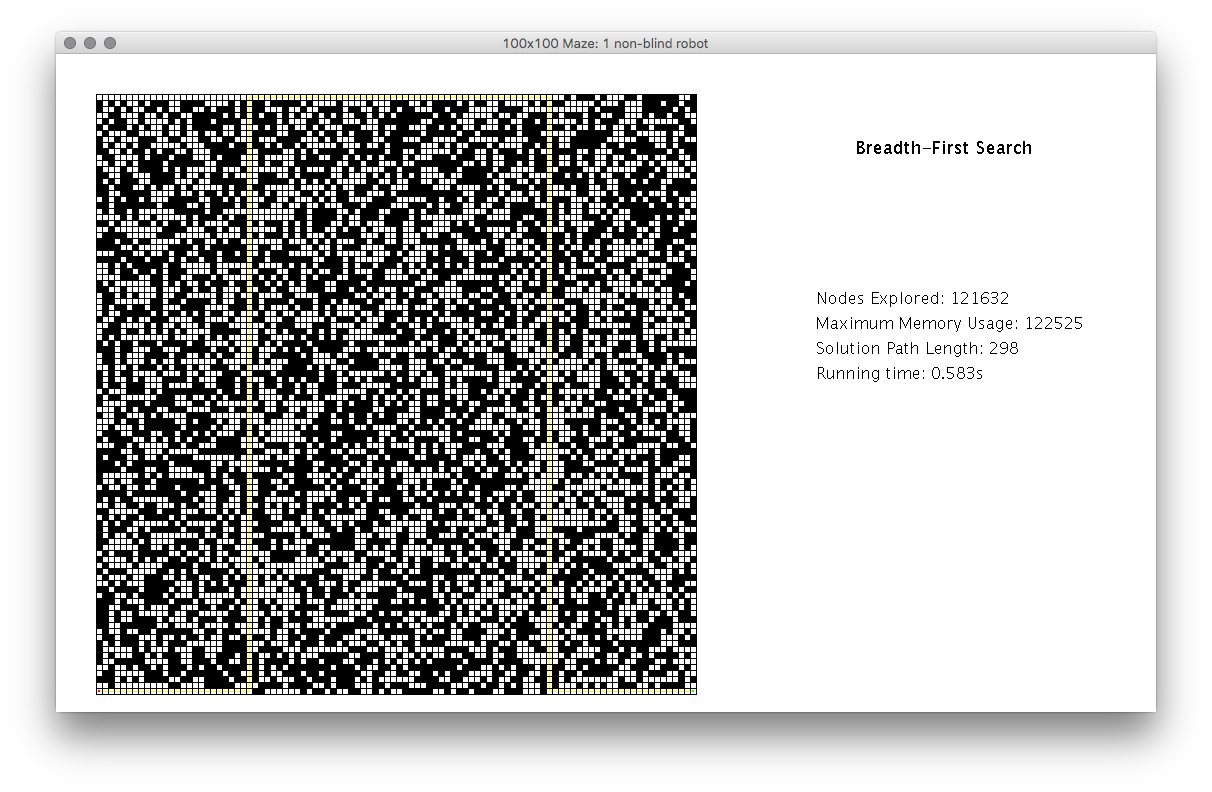
\includegraphics[width=1\linewidth]{./figures/BFS-maze100x100.png}
\cprotect\caption{An example of BFS solving a 100x100 maze with a non-blind robot with initial position at $(0,0)$ and goal at $(99,0)$. The yellow path represents the solution path.}
\end{figure}

\begin{figure}[!htb]
\label{fig:asearch}
\centering
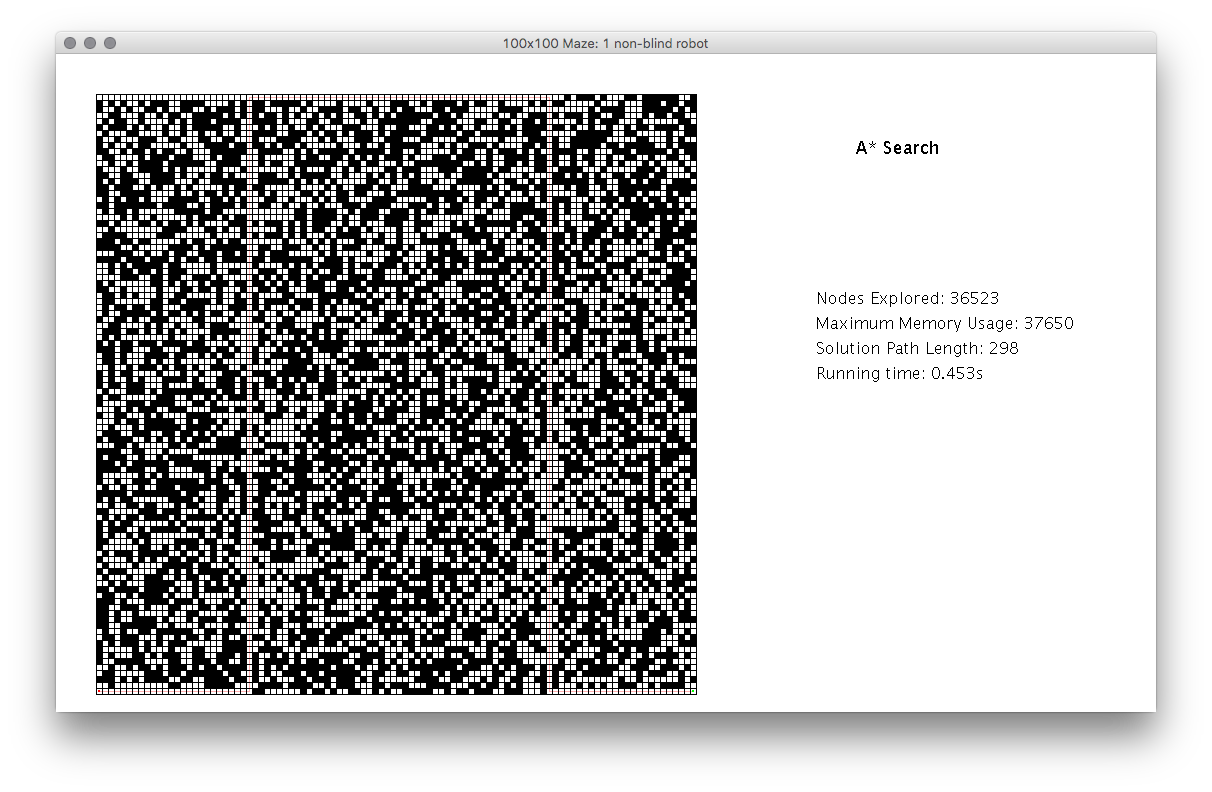
\includegraphics[width=1\linewidth]{./figures/A-maze100x100.png}
\cprotect\caption{An example of A*S solving a 100x100 maze with a non-blind robot with initial position at $(0,0)$ and goal at $(99,0)$. The pink path represents the solution path.}
\end{figure}

\begin{figure}[!htb]
\label{fig:blind}
\centering
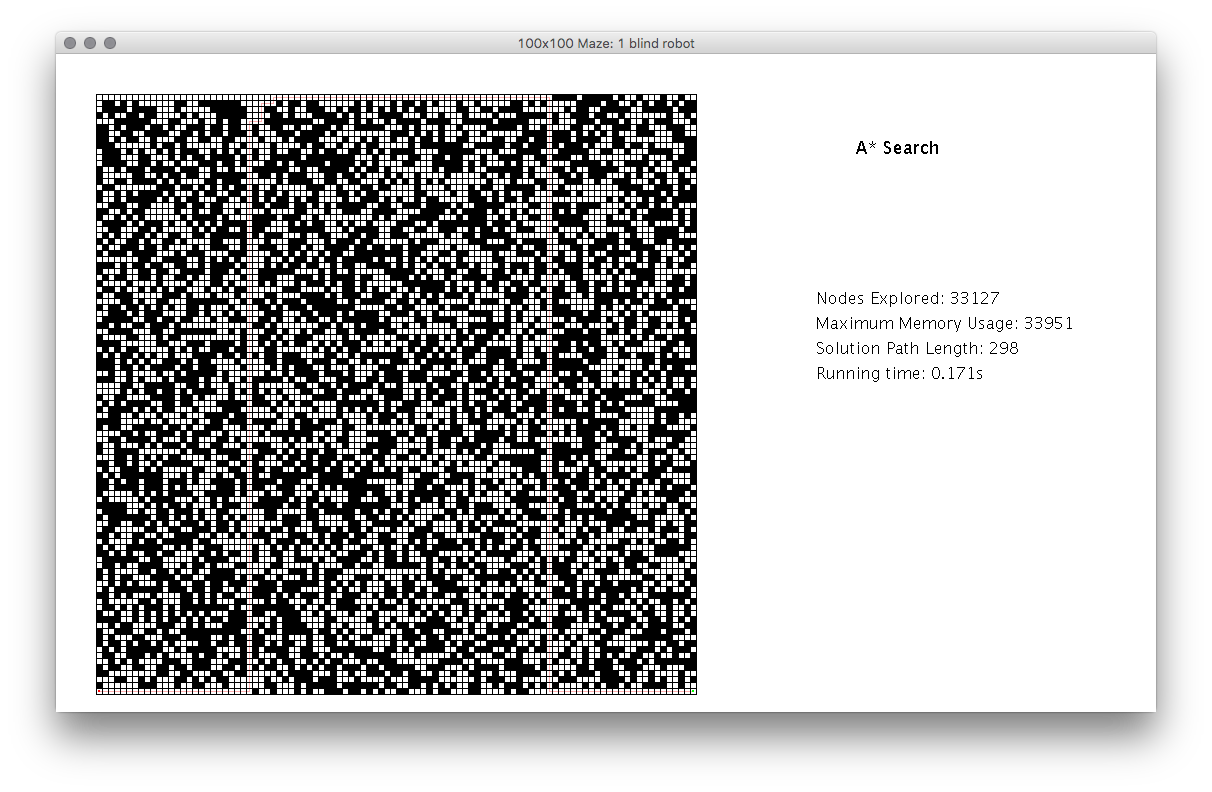
\includegraphics[width=1\linewidth]{./figures/A-blind-maze100x100.png}
\cprotect\caption{An example of A*S solving a 100x100 maze with a blind robot with initial position at $(0,0)$ and goal at $(99,0)$. The pink path represents the solution path.}
\end{figure}

\end{document}